\begin{equation}
Q(\mathbf{x}) = \sum_{i=1}^n \left( \frac{x_i}{\sigma_0} \right)^2
\end{equation}

Note que para $\mathbf{x}^T = (x_1, \ldots, x_n)^T$, $Q(\mathbf{x}) \overset{H_0}{\sim} \chi^2_{n}$.

Assim, o teste t\'{\i}pico: Rejeitamos $H_0$ se
\[
\mathbf{x} \notin R_c = \left\{ \mathbf{x} \in \mathcal{X} : Q(\mathbf{x}) < \chi^2_{n,\alpha} \right\},
\]
em que $\chi^2_{n,\alpha}$ \'e solu\c{c}\~ao de, para $Q \sim \chi^2_n$,
\[
P_{H_0} \left( Q < \chi^2_{n,\alpha} \right) = \alpha.
\]

\begin{center}
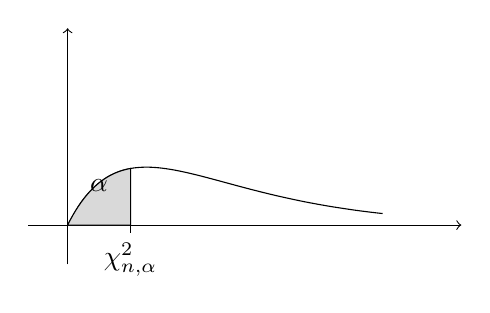
\begin{tikzpicture}[scale=1.0]
\draw[->] (-0.5,0) -- (5,0);
\draw[->] (0,-0.5) -- (0,2.5);
\draw[domain=0:4,smooth,variable=\x] plot ({\x},{2*\x*exp(-\x)});
\draw[fill=gray!30] (0,0) -- plot[domain=0:0.8] ({\x},{2*\x*exp(-\x)}) -- (0.8,0) -- cycle;
\node at (0.4,0.5) {$\alpha$};
\draw (0.8,0) -- (0.8,-0.1) node[below] {$\chi^2_{n,\alpha}$};
\end{tikzpicture}
\end{center}

\noindent \textbf{Aula 21 (09/06/2023)} \\

Teste UMP via raz\~ao de verossimilhan\c{c}a.

Seja $\mathbf{X} = (X_1, \ldots, X_n)^T$ uma a.a. de $X$ tendo fdp (ou fmp) $f(x; \theta)$ para $x \in \mathcal{X} \subset \mathbb{R}$ e $\theta \in \Theta \subset \mathbb{R}$.

\noindent Defini\c{c}\~ao (raz\~ao de verossimilhan\c{c}a monotona - RVM): A fam\'{\i}lia
\[
\left\{ f(x|\theta), \ \theta \in \Theta \right\}
\]
